\documentclass[twoside]{book}

% Packages required by doxygen
\usepackage{fixltx2e}
\usepackage{calc}
\usepackage{doxygen}
\usepackage[export]{adjustbox} % also loads graphicx
\usepackage{graphicx}
\usepackage[utf8]{inputenc}
\usepackage{makeidx}
\usepackage{multicol}
\usepackage{multirow}
\PassOptionsToPackage{warn}{textcomp}
\usepackage{textcomp}
\usepackage[nointegrals]{wasysym}
\usepackage[table]{xcolor}

% Font selection
\usepackage[T1]{fontenc}
\usepackage[scaled=.90]{helvet}
\usepackage{courier}
\usepackage{amssymb}
\usepackage{sectsty}
\renewcommand{\familydefault}{\sfdefault}
\allsectionsfont{%
  \fontseries{bc}\selectfont%
  \color{darkgray}%
}
\renewcommand{\DoxyLabelFont}{%
  \fontseries{bc}\selectfont%
  \color{darkgray}%
}
\newcommand{\+}{\discretionary{\mbox{\scriptsize$\hookleftarrow$}}{}{}}

% Page & text layout
\usepackage{geometry}
\geometry{%
  a4paper,%
  top=2.5cm,%
  bottom=2.5cm,%
  left=2.5cm,%
  right=2.5cm%
}
\tolerance=750
\hfuzz=15pt
\hbadness=750
\setlength{\emergencystretch}{15pt}
\setlength{\parindent}{0cm}
\setlength{\parskip}{3ex plus 2ex minus 2ex}
\makeatletter
\renewcommand{\paragraph}{%
  \@startsection{paragraph}{4}{0ex}{-1.0ex}{1.0ex}{%
    \normalfont\normalsize\bfseries\SS@parafont%
  }%
}
\renewcommand{\subparagraph}{%
  \@startsection{subparagraph}{5}{0ex}{-1.0ex}{1.0ex}{%
    \normalfont\normalsize\bfseries\SS@subparafont%
  }%
}
\makeatother

% Headers & footers
\usepackage{fancyhdr}
\pagestyle{fancyplain}
\fancyhead[LE]{\fancyplain{}{\bfseries\thepage}}
\fancyhead[CE]{\fancyplain{}{}}
\fancyhead[RE]{\fancyplain{}{\bfseries\leftmark}}
\fancyhead[LO]{\fancyplain{}{\bfseries\rightmark}}
\fancyhead[CO]{\fancyplain{}{}}
\fancyhead[RO]{\fancyplain{}{\bfseries\thepage}}
\fancyfoot[LE]{\fancyplain{}{}}
\fancyfoot[CE]{\fancyplain{}{}}
\fancyfoot[RE]{\fancyplain{}{\bfseries\scriptsize Generated by Doxygen }}
\fancyfoot[LO]{\fancyplain{}{\bfseries\scriptsize Generated by Doxygen }}
\fancyfoot[CO]{\fancyplain{}{}}
\fancyfoot[RO]{\fancyplain{}{}}
\renewcommand{\footrulewidth}{0.4pt}
\renewcommand{\chaptermark}[1]{%
  \markboth{#1}{}%
}
\renewcommand{\sectionmark}[1]{%
  \markright{\thesection\ #1}%
}

% Indices & bibliography
\usepackage{natbib}
\usepackage[titles]{tocloft}
\setcounter{tocdepth}{3}
\setcounter{secnumdepth}{5}
\makeindex

% Hyperlinks (required, but should be loaded last)
\usepackage{ifpdf}
\ifpdf
  \usepackage[pdftex,pagebackref=true]{hyperref}
\else
  \usepackage[ps2pdf,pagebackref=true]{hyperref}
\fi
\hypersetup{%
  colorlinks=true,%
  linkcolor=blue,%
  citecolor=blue,%
  unicode%
}

% Custom commands
\newcommand{\clearemptydoublepage}{%
  \newpage{\pagestyle{empty}\cleardoublepage}%
}

\usepackage{caption}
\captionsetup{labelsep=space,justification=centering,font={bf},singlelinecheck=off,skip=4pt,position=top}

%===== C O N T E N T S =====

\begin{document}

% Titlepage & ToC
\hypersetup{pageanchor=false,
             bookmarksnumbered=true,
             pdfencoding=unicode
            }
\pagenumbering{roman}
\begin{titlepage}
\vspace*{7cm}
\begin{center}%
{\Large My Project }\\
\vspace*{1cm}
{\large Generated by Doxygen 1.8.11}\\
\end{center}
\end{titlepage}
\clearemptydoublepage
\tableofcontents
\clearemptydoublepage
\pagenumbering{arabic}
\hypersetup{pageanchor=true}

%--- Begin generated contents ---
\chapter{Namespace Index}
\section{Namespace List}
Here is a list of all namespaces with brief descriptions\+:\begin{DoxyCompactList}
\item\contentsline{section}{\hyperlink{namespacemyFunc}{my\+Func} }{\pageref{namespacemyFunc}}{}
\item\contentsline{section}{\hyperlink{namespacestd}{std} }{\pageref{namespacestd}}{}
\end{DoxyCompactList}

\chapter{Hierarchical Index}
\section{Class Hierarchy}
This inheritance list is sorted roughly, but not completely, alphabetically\+:\begin{DoxyCompactList}
\item \contentsline{section}{byteview$<$ T $>$}{\pageref{unionbyteview}}{}
\item false\+\_\+type\begin{DoxyCompactList}
\item \contentsline{section}{my\+Func\+:\+:is\+\_\+one\+\_\+of$<$ std\+:\+:tuple\+\_\+element$<$ 0, V $>$\+:\+:type, std\+:\+:tuple\+\_\+element$<$ S, V $>$\+:\+:type, S-\/1, V $>$}{\pageref{structmyFunc_1_1is__one__of}}{}
\begin{DoxyCompactList}
\item \contentsline{section}{my\+Func\+:\+:is\+\_\+one\+\_\+of$<$ T, T, S, V $>$}{\pageref{structmyFunc_1_1is__one__of_3_01T_00_01T_00_01S_00_01V_01_4}}{}
\end{DoxyCompactList}
\item \contentsline{section}{my\+Func\+:\+:is\+\_\+one\+\_\+of$<$ T, U, S, V $>$}{\pageref{structmyFunc_1_1is__one__of}}{}
\item \contentsline{section}{my\+Func\+:\+:Is\+Tuple\+Impl$<$ T $>$}{\pageref{structmyFunc_1_1IsTupleImpl}}{}
\end{DoxyCompactList}
\item \contentsline{section}{print$<$ T, is\+\_\+integral, is\+\_\+object, is\+\_\+tuple $>$}{\pageref{structprint}}{}
\item \contentsline{section}{print$<$ T, false, true, false $>$}{\pageref{structprint_3_01T_00_01false_00_01true_00_01false_01_4}}{}
\item \contentsline{section}{print$<$ T, false, true, true $>$}{\pageref{structprint_3_01T_00_01false_00_01true_00_01true_01_4}}{}
\item \contentsline{section}{print$<$ T, true, false, false $>$}{\pageref{structprint_3_01T_00_01true_00_01false_00_01false_01_4}}{}
\item true\+\_\+type\begin{DoxyCompactList}
\item \contentsline{section}{my\+Func\+:\+:is\+\_\+one\+\_\+of$<$ T, T, 1, V $>$}{\pageref{structmyFunc_1_1is__one__of_3_01T_00_01T_00_011_00_01V_01_4}}{}
\item \contentsline{section}{my\+Func\+:\+:Is\+Tuple\+Impl$<$ std\+:\+:tuple$<$ U... $>$ $>$}{\pageref{structmyFunc_1_1IsTupleImpl_3_01std_1_1tuple_3_01U_8_8_8_01_4_01_4}}{}
\end{DoxyCompactList}
\item \contentsline{section}{my\+Func\+:\+:Tuple\+Printer$<$ Tuple, N $>$}{\pageref{structmyFunc_1_1TuplePrinter}}{}
\item \contentsline{section}{my\+Func\+:\+:Tuple\+Printer$<$ Tuple, 1 $>$}{\pageref{structmyFunc_1_1TuplePrinter_3_01Tuple_00_011_01_4}}{}
\end{DoxyCompactList}

\chapter{Class Index}
\section{Class List}
Here are the classes, structs, unions and interfaces with brief descriptions\+:\begin{DoxyCompactList}
\item\contentsline{section}{\hyperlink{unionbyteview}{byteview$<$ T $>$} }{\pageref{unionbyteview}}{}
\item\contentsline{section}{\hyperlink{structmyFunc_1_1is__one__of}{my\+Func\+::is\+\_\+one\+\_\+of$<$ T, U, i, V $>$} }{\pageref{structmyFunc_1_1is__one__of}}{}
\item\contentsline{section}{\hyperlink{structmyFunc_1_1is__one__of_3_01T_00_01T_00_011_00_01V_01_4}{my\+Func\+::is\+\_\+one\+\_\+of$<$ T, T, 1, V $>$} }{\pageref{structmyFunc_1_1is__one__of_3_01T_00_01T_00_011_00_01V_01_4}}{}
\item\contentsline{section}{\hyperlink{structmyFunc_1_1is__one__of_3_01T_00_01T_00_01i_00_01V_01_4}{my\+Func\+::is\+\_\+one\+\_\+of$<$ T, T, i, V $>$} }{\pageref{structmyFunc_1_1is__one__of_3_01T_00_01T_00_01i_00_01V_01_4}}{}
\item\contentsline{section}{\hyperlink{structmyFunc_1_1IsTupleImpl}{my\+Func\+::\+Is\+Tuple\+Impl$<$ T $>$} }{\pageref{structmyFunc_1_1IsTupleImpl}}{}
\item\contentsline{section}{\hyperlink{structmyFunc_1_1IsTupleImpl_3_01std_1_1tuple_3_01U_8_8_8_01_4_01_4}{my\+Func\+::\+Is\+Tuple\+Impl$<$ std\+::tuple$<$ U... $>$ $>$} }{\pageref{structmyFunc_1_1IsTupleImpl_3_01std_1_1tuple_3_01U_8_8_8_01_4_01_4}}{}
\item\contentsline{section}{\hyperlink{structprint}{print$<$ T, is\+\_\+integral, is\+\_\+object, is\+\_\+tuple $>$} }{\pageref{structprint}}{}
\item\contentsline{section}{\hyperlink{structprint_3_01T_00_01false_00_01true_00_01false_01_4}{print$<$ T, false, true, false $>$} }{\pageref{structprint_3_01T_00_01false_00_01true_00_01false_01_4}}{}
\item\contentsline{section}{\hyperlink{structprint_3_01T_00_01false_00_01true_00_01true_01_4}{print$<$ T, false, true, true $>$} }{\pageref{structprint_3_01T_00_01false_00_01true_00_01true_01_4}}{}
\item\contentsline{section}{\hyperlink{structprint_3_01T_00_01true_00_01false_00_01false_01_4}{print$<$ T, true, false, false $>$} }{\pageref{structprint_3_01T_00_01true_00_01false_00_01false_01_4}}{}
\item\contentsline{section}{\hyperlink{structmyFunc_1_1TuplePrinter}{my\+Func\+::\+Tuple\+Printer$<$ Tuple, N $>$} }{\pageref{structmyFunc_1_1TuplePrinter}}{}
\item\contentsline{section}{\hyperlink{structmyFunc_1_1TuplePrinter_3_01Tuple_00_011_01_4}{my\+Func\+::\+Tuple\+Printer$<$ Tuple, 1 $>$} }{\pageref{structmyFunc_1_1TuplePrinter_3_01Tuple_00_011_01_4}}{}
\end{DoxyCompactList}

\chapter{File Index}
\section{File List}
Here is a list of all files with brief descriptions\+:\begin{DoxyCompactList}
\item\contentsline{section}{\hyperlink{main_8cpp}{main.\+cpp} }{\pageref{main_8cpp}}{}
\item\contentsline{section}{\hyperlink{print__ip_8cpp}{print\+\_\+ip.\+cpp} }{\pageref{print__ip_8cpp}}{}
\item\contentsline{section}{\hyperlink{test__ip__print_8cpp}{test\+\_\+ip\+\_\+print.\+cpp} }{\pageref{test__ip__print_8cpp}}{}
\end{DoxyCompactList}

\chapter{Namespace Documentation}
\hypertarget{namespacemyFunc}{}\section{my\+Func Namespace Reference}
\label{namespacemyFunc}\index{my\+Func@{my\+Func}}
\subsection*{Classes}
\begin{DoxyCompactItemize}
\item 
struct \hyperlink{structmyFunc_1_1is__one__of}{is\+\_\+one\+\_\+of}
\item 
struct \hyperlink{structmyFunc_1_1is__one__of_3_01T_00_01T_00_011_00_01V_01_4}{is\+\_\+one\+\_\+of$<$ T, T, 1, V $>$}
\item 
struct \hyperlink{structmyFunc_1_1is__one__of_3_01T_00_01T_00_01S_00_01V_01_4}{is\+\_\+one\+\_\+of$<$ T, T, S, V $>$}
\item 
struct \hyperlink{structmyFunc_1_1IsTupleImpl}{Is\+Tuple\+Impl}
\item 
struct \hyperlink{structmyFunc_1_1IsTupleImpl_3_01std_1_1tuple_3_01U_8_8_8_01_4_01_4}{Is\+Tuple\+Impl$<$ std\+::tuple$<$ U... $>$ $>$}
\item 
struct \hyperlink{structmyFunc_1_1TuplePrinter}{Tuple\+Printer}
\item 
struct \hyperlink{structmyFunc_1_1TuplePrinter_3_01Tuple_00_011_01_4}{Tuple\+Printer$<$ Tuple, 1 $>$}
\end{DoxyCompactItemize}
\subsection*{Functions}
\begin{DoxyCompactItemize}
\item 
{\footnotesize template$<$typename T $>$ }\\constexpr bool \hyperlink{namespacemyFunc_afe24a25839d94fd3368128576589722a}{is\+\_\+tuple\+\_\+v} ()
\item 
{\footnotesize template$<$typename T $>$ }\\std\+::enable\+\_\+if\+\_\+t$<$ std\+::is\+\_\+compound$<$ T $>$\+::value, std\+::string $>$ \hyperlink{namespacemyFunc_a3f0d86a5a675a3cdfae97fe12405c6a9}{all\+\_\+to\+\_\+sting} (T t)
\item 
{\footnotesize template$<$typename T $>$ }\\std\+::enable\+\_\+if\+\_\+t$<$ \hyperlink{namespacestd_a824c5eb1a7e8aafa382dc9af3329a9e8}{std\+::is\+\_\+integral\+\_\+v}$<$ T $>$, std\+::string $>$ \hyperlink{namespacemyFunc_a501f8e9903912dcbd57e865a214c6568}{all\+\_\+to\+\_\+sting} (T t)
\item 
{\footnotesize template$<$class... Args$>$ }\\void \hyperlink{namespacemyFunc_a6588b7e742bf09aefea7d531f5c8ca6e}{tuple\+\_\+print} (const std\+::tuple$<$ Args... $>$ \&t)
\end{DoxyCompactItemize}
\subsection*{Variables}
\begin{DoxyCompactItemize}
\item 
{\footnotesize template$<$typename T , typename U , size\+\_\+t S, typename V $>$ }\\constexpr bool \hyperlink{namespacemyFunc_aa757a804546f113b7cadf75b0a1ec7e1}{is\+\_\+one\+\_\+of\+\_\+v} = \hyperlink{structmyFunc_1_1is__one__of}{is\+\_\+one\+\_\+of}$<$T,U,S,V$>$\+::value
\end{DoxyCompactItemize}


\subsection{Function Documentation}
\index{my\+Func@{my\+Func}!all\+\_\+to\+\_\+sting@{all\+\_\+to\+\_\+sting}}
\index{all\+\_\+to\+\_\+sting@{all\+\_\+to\+\_\+sting}!my\+Func@{my\+Func}}
\subsubsection[{\texorpdfstring{all\+\_\+to\+\_\+sting(\+T t)}{all_to_sting(T t)}}]{\setlength{\rightskip}{0pt plus 5cm}template$<$typename T $>$ std\+::enable\+\_\+if\+\_\+t$<$std\+::is\+\_\+compound$<$T$>$\+::value, std\+::string$>$ my\+Func\+::all\+\_\+to\+\_\+sting (
\begin{DoxyParamCaption}
\item[{T}]{t}
\end{DoxyParamCaption}
)}\hypertarget{namespacemyFunc_a3f0d86a5a675a3cdfae97fe12405c6a9}{}\label{namespacemyFunc_a3f0d86a5a675a3cdfae97fe12405c6a9}
\index{my\+Func@{my\+Func}!all\+\_\+to\+\_\+sting@{all\+\_\+to\+\_\+sting}}
\index{all\+\_\+to\+\_\+sting@{all\+\_\+to\+\_\+sting}!my\+Func@{my\+Func}}
\subsubsection[{\texorpdfstring{all\+\_\+to\+\_\+sting(\+T t)}{all_to_sting(T t)}}]{\setlength{\rightskip}{0pt plus 5cm}template$<$typename T $>$ std\+::enable\+\_\+if\+\_\+t$<${\bf std\+::is\+\_\+integral\+\_\+v}$<$T$>$, std\+::string$>$ my\+Func\+::all\+\_\+to\+\_\+sting (
\begin{DoxyParamCaption}
\item[{T}]{t}
\end{DoxyParamCaption}
)}\hypertarget{namespacemyFunc_a501f8e9903912dcbd57e865a214c6568}{}\label{namespacemyFunc_a501f8e9903912dcbd57e865a214c6568}
\index{my\+Func@{my\+Func}!is\+\_\+tuple\+\_\+v@{is\+\_\+tuple\+\_\+v}}
\index{is\+\_\+tuple\+\_\+v@{is\+\_\+tuple\+\_\+v}!my\+Func@{my\+Func}}
\subsubsection[{\texorpdfstring{is\+\_\+tuple\+\_\+v()}{is_tuple_v()}}]{\setlength{\rightskip}{0pt plus 5cm}template$<$typename T $>$ constexpr bool my\+Func\+::is\+\_\+tuple\+\_\+v (
\begin{DoxyParamCaption}
{}
\end{DoxyParamCaption}
)}\hypertarget{namespacemyFunc_afe24a25839d94fd3368128576589722a}{}\label{namespacemyFunc_afe24a25839d94fd3368128576589722a}
\index{my\+Func@{my\+Func}!tuple\+\_\+print@{tuple\+\_\+print}}
\index{tuple\+\_\+print@{tuple\+\_\+print}!my\+Func@{my\+Func}}
\subsubsection[{\texorpdfstring{tuple\+\_\+print(const std\+::tuple$<$ Args... $>$ \&t)}{tuple_print(const std::tuple< Args... > &t)}}]{\setlength{\rightskip}{0pt plus 5cm}template$<$class... Args$>$ void my\+Func\+::tuple\+\_\+print (
\begin{DoxyParamCaption}
\item[{const std\+::tuple$<$ Args... $>$ \&}]{t}
\end{DoxyParamCaption}
)}\hypertarget{namespacemyFunc_a6588b7e742bf09aefea7d531f5c8ca6e}{}\label{namespacemyFunc_a6588b7e742bf09aefea7d531f5c8ca6e}


\subsection{Variable Documentation}
\index{my\+Func@{my\+Func}!is\+\_\+one\+\_\+of\+\_\+v@{is\+\_\+one\+\_\+of\+\_\+v}}
\index{is\+\_\+one\+\_\+of\+\_\+v@{is\+\_\+one\+\_\+of\+\_\+v}!my\+Func@{my\+Func}}
\subsubsection[{\texorpdfstring{is\+\_\+one\+\_\+of\+\_\+v}{is_one_of_v}}]{\setlength{\rightskip}{0pt plus 5cm}template$<$typename T , typename U , size\+\_\+t S, typename V $>$ constexpr bool my\+Func\+::is\+\_\+one\+\_\+of\+\_\+v = {\bf is\+\_\+one\+\_\+of}$<$T,U,S,V$>$\+::value}\hypertarget{namespacemyFunc_aa757a804546f113b7cadf75b0a1ec7e1}{}\label{namespacemyFunc_aa757a804546f113b7cadf75b0a1ec7e1}

\hypertarget{namespacestd}{}\section{std Namespace Reference}
\label{namespacestd}\index{std@{std}}
\subsection*{Variables}
\begin{DoxyCompactItemize}
\item 
{\footnotesize template$<$typename T $>$ }\\constexpr bool \hyperlink{namespacestd_a824c5eb1a7e8aafa382dc9af3329a9e8}{is\+\_\+integral\+\_\+v} = is\+\_\+integral$<$T$>$\+::value
\item 
{\footnotesize template$<$typename T $>$ }\\constexpr bool \hyperlink{namespacestd_ae1e905cdb2694181466fae8f8dd8f8e8}{is\+\_\+compound\+\_\+v} = is\+\_\+compound$<$T$>$\+::value
\end{DoxyCompactItemize}


\subsection{Variable Documentation}
\index{std@{std}!is\+\_\+compound\+\_\+v@{is\+\_\+compound\+\_\+v}}
\index{is\+\_\+compound\+\_\+v@{is\+\_\+compound\+\_\+v}!std@{std}}
\subsubsection[{\texorpdfstring{is\+\_\+compound\+\_\+v}{is_compound_v}}]{\setlength{\rightskip}{0pt plus 5cm}template$<$typename T $>$ constexpr bool std\+::is\+\_\+compound\+\_\+v = is\+\_\+compound$<$T$>$\+::value}\hypertarget{namespacestd_ae1e905cdb2694181466fae8f8dd8f8e8}{}\label{namespacestd_ae1e905cdb2694181466fae8f8dd8f8e8}
\index{std@{std}!is\+\_\+integral\+\_\+v@{is\+\_\+integral\+\_\+v}}
\index{is\+\_\+integral\+\_\+v@{is\+\_\+integral\+\_\+v}!std@{std}}
\subsubsection[{\texorpdfstring{is\+\_\+integral\+\_\+v}{is_integral_v}}]{\setlength{\rightskip}{0pt plus 5cm}template$<$typename T $>$ constexpr bool std\+::is\+\_\+integral\+\_\+v = is\+\_\+integral$<$T$>$\+::value}\hypertarget{namespacestd_a824c5eb1a7e8aafa382dc9af3329a9e8}{}\label{namespacestd_a824c5eb1a7e8aafa382dc9af3329a9e8}

\chapter{Class Documentation}
\hypertarget{unionbyteview}{}\section{byteview$<$ T $>$ Union Template Reference}
\label{unionbyteview}\index{byteview$<$ T $>$@{byteview$<$ T $>$}}


Collaboration diagram for byteview$<$ T $>$\+:
\nopagebreak
\begin{figure}[H]
\begin{center}
\leavevmode
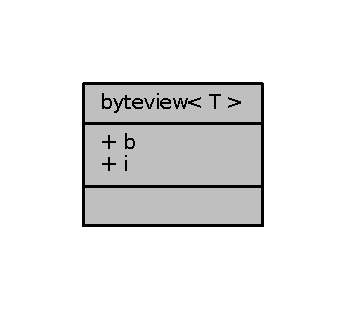
\includegraphics[width=166pt]{unionbyteview__coll__graph}
\end{center}
\end{figure}
\subsection*{Public Attributes}
\begin{DoxyCompactItemize}
\item 
unsigned char \hyperlink{unionbyteview_af86288b3e2724623c6a8836c07b26d28}{b} \mbox{[}sizeof(T)\mbox{]}
\item 
T \hyperlink{unionbyteview_a34c79afd8afd71191848bd8fa06fd286}{i}
\end{DoxyCompactItemize}


\subsection{Member Data Documentation}
\index{byteview@{byteview}!b@{b}}
\index{b@{b}!byteview@{byteview}}
\subsubsection[{\texorpdfstring{b}{b}}]{\setlength{\rightskip}{0pt plus 5cm}template$<$typename T$>$ unsigned char {\bf byteview}$<$ T $>$\+::b\mbox{[}sizeof(T)\mbox{]}}\hypertarget{unionbyteview_af86288b3e2724623c6a8836c07b26d28}{}\label{unionbyteview_af86288b3e2724623c6a8836c07b26d28}
\index{byteview@{byteview}!i@{i}}
\index{i@{i}!byteview@{byteview}}
\subsubsection[{\texorpdfstring{i}{i}}]{\setlength{\rightskip}{0pt plus 5cm}template$<$typename T$>$ T {\bf byteview}$<$ T $>$\+::i}\hypertarget{unionbyteview_a34c79afd8afd71191848bd8fa06fd286}{}\label{unionbyteview_a34c79afd8afd71191848bd8fa06fd286}


The documentation for this union was generated from the following file\+:\begin{DoxyCompactItemize}
\item 
\hyperlink{print__ip_8cpp}{print\+\_\+ip.\+cpp}\end{DoxyCompactItemize}

\hypertarget{structmyFunc_1_1is__one__of}{}\section{my\+Func\+:\+:is\+\_\+one\+\_\+of$<$ T, U, i, V $>$ Struct Template Reference}
\label{structmyFunc_1_1is__one__of}\index{my\+Func\+::is\+\_\+one\+\_\+of$<$ T, U, i, V $>$@{my\+Func\+::is\+\_\+one\+\_\+of$<$ T, U, i, V $>$}}


Inheritance diagram for my\+Func\+:\+:is\+\_\+one\+\_\+of$<$ T, U, i, V $>$\+:
\nopagebreak
\begin{figure}[H]
\begin{center}
\leavevmode
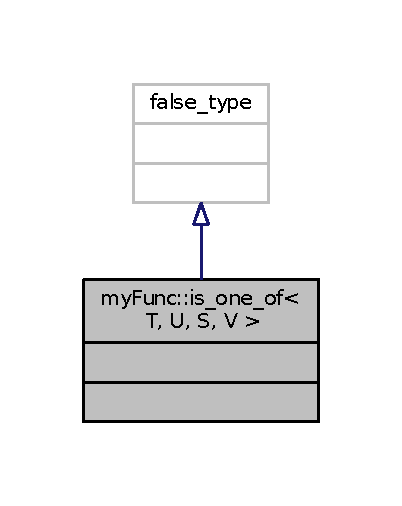
\includegraphics[width=193pt]{structmyFunc_1_1is__one__of__inherit__graph}
\end{center}
\end{figure}


Collaboration diagram for my\+Func\+:\+:is\+\_\+one\+\_\+of$<$ T, U, i, V $>$\+:
\nopagebreak
\begin{figure}[H]
\begin{center}
\leavevmode
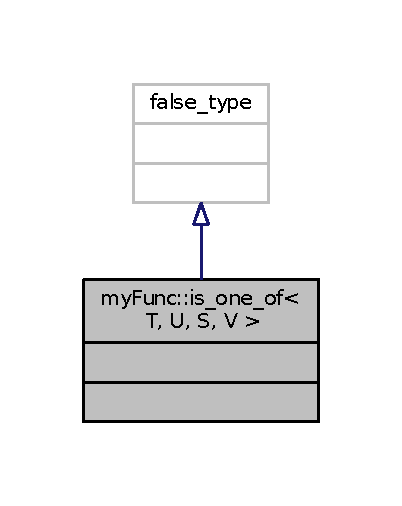
\includegraphics[width=193pt]{structmyFunc_1_1is__one__of__coll__graph}
\end{center}
\end{figure}


The documentation for this struct was generated from the following file\+:\begin{DoxyCompactItemize}
\item 
\hyperlink{print__ip_8cpp}{print\+\_\+ip.\+cpp}\end{DoxyCompactItemize}

\hypertarget{structmyFunc_1_1is__one__of_3_01T_00_01T_00_011_00_01V_01_4}{}\section{my\+Func\+:\+:is\+\_\+one\+\_\+of$<$ T, T, 1, V $>$ Struct Template Reference}
\label{structmyFunc_1_1is__one__of_3_01T_00_01T_00_011_00_01V_01_4}\index{my\+Func\+::is\+\_\+one\+\_\+of$<$ T, T, 1, V $>$@{my\+Func\+::is\+\_\+one\+\_\+of$<$ T, T, 1, V $>$}}


Inheritance diagram for my\+Func\+:\+:is\+\_\+one\+\_\+of$<$ T, T, 1, V $>$\+:
% FIG 0


Collaboration diagram for my\+Func\+:\+:is\+\_\+one\+\_\+of$<$ T, T, 1, V $>$\+:
% FIG 1


The documentation for this struct was generated from the following file\+:\begin{DoxyCompactItemize}
\item 
\hyperlink{print__ip_8cpp}{print\+\_\+ip.\+cpp}\end{DoxyCompactItemize}

\hypertarget{structmyFunc_1_1is__one__of_3_01T_00_01T_00_01S_00_01V_01_4}{}\section{my\+Func\+:\+:is\+\_\+one\+\_\+of$<$ T, T, S, V $>$ Struct Template Reference}
\label{structmyFunc_1_1is__one__of_3_01T_00_01T_00_01S_00_01V_01_4}\index{my\+Func\+::is\+\_\+one\+\_\+of$<$ T, T, S, V $>$@{my\+Func\+::is\+\_\+one\+\_\+of$<$ T, T, S, V $>$}}


Inheritance diagram for my\+Func\+:\+:is\+\_\+one\+\_\+of$<$ T, T, S, V $>$\+:
% FIG 0


Collaboration diagram for my\+Func\+:\+:is\+\_\+one\+\_\+of$<$ T, T, S, V $>$\+:
% FIG 1


The documentation for this struct was generated from the following file\+:\begin{DoxyCompactItemize}
\item 
\hyperlink{print__ip_8cpp}{print\+\_\+ip.\+cpp}\end{DoxyCompactItemize}

\hypertarget{structmyFunc_1_1IsTupleImpl}{}\section{my\+Func\+:\+:Is\+Tuple\+Impl$<$ T $>$ Struct Template Reference}
\label{structmyFunc_1_1IsTupleImpl}\index{my\+Func\+::\+Is\+Tuple\+Impl$<$ T $>$@{my\+Func\+::\+Is\+Tuple\+Impl$<$ T $>$}}


Inheritance diagram for my\+Func\+:\+:Is\+Tuple\+Impl$<$ T $>$\+:
\nopagebreak
\begin{figure}[H]
\begin{center}
\leavevmode
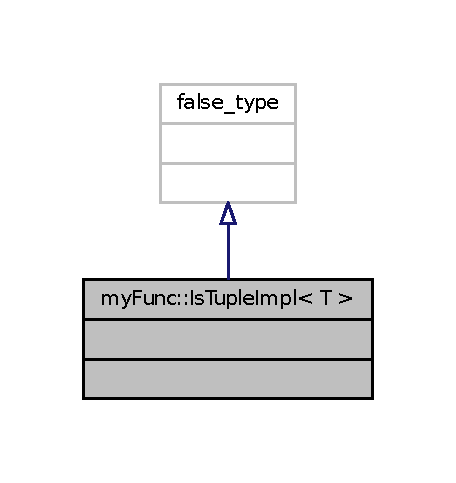
\includegraphics[width=219pt]{structmyFunc_1_1IsTupleImpl__inherit__graph}
\end{center}
\end{figure}


Collaboration diagram for my\+Func\+:\+:Is\+Tuple\+Impl$<$ T $>$\+:
\nopagebreak
\begin{figure}[H]
\begin{center}
\leavevmode
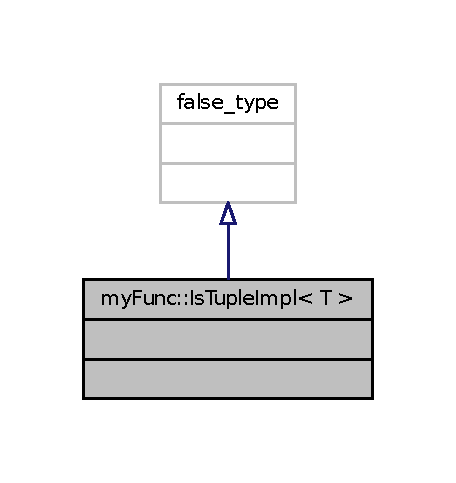
\includegraphics[width=219pt]{structmyFunc_1_1IsTupleImpl__coll__graph}
\end{center}
\end{figure}


The documentation for this struct was generated from the following file\+:\begin{DoxyCompactItemize}
\item 
\hyperlink{print__ip_8cpp}{print\+\_\+ip.\+cpp}\end{DoxyCompactItemize}

\hypertarget{structmyFunc_1_1IsTupleImpl_3_01std_1_1tuple_3_01U_8_8_8_01_4_01_4}{}\section{my\+Func\+:\+:Is\+Tuple\+Impl$<$ std\+:\+:tuple$<$ U... $>$ $>$ Struct Template Reference}
\label{structmyFunc_1_1IsTupleImpl_3_01std_1_1tuple_3_01U_8_8_8_01_4_01_4}\index{my\+Func\+::\+Is\+Tuple\+Impl$<$ std\+::tuple$<$ U... $>$ $>$@{my\+Func\+::\+Is\+Tuple\+Impl$<$ std\+::tuple$<$ U... $>$ $>$}}


Inheritance diagram for my\+Func\+:\+:Is\+Tuple\+Impl$<$ std\+:\+:tuple$<$ U... $>$ $>$\+:
% FIG 0


Collaboration diagram for my\+Func\+:\+:Is\+Tuple\+Impl$<$ std\+:\+:tuple$<$ U... $>$ $>$\+:
% FIG 1


The documentation for this struct was generated from the following file\+:\begin{DoxyCompactItemize}
\item 
\hyperlink{print__ip_8cpp}{print\+\_\+ip.\+cpp}\end{DoxyCompactItemize}

\hypertarget{structprint}{}\section{print$<$ T, is\+\_\+integral, is\+\_\+object, is\+\_\+tuple $>$ Struct Template Reference}
\label{structprint}\index{print$<$ T, is\+\_\+integral, is\+\_\+object, is\+\_\+tuple $>$@{print$<$ T, is\+\_\+integral, is\+\_\+object, is\+\_\+tuple $>$}}


Collaboration diagram for print$<$ T, is\+\_\+integral, is\+\_\+object, is\+\_\+tuple $>$\+:
\nopagebreak
\begin{figure}[H]
\begin{center}
\leavevmode
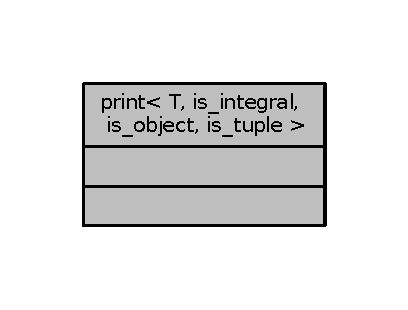
\includegraphics[width=196pt]{structprint__coll__graph}
\end{center}
\end{figure}


The documentation for this struct was generated from the following file\+:\begin{DoxyCompactItemize}
\item 
\hyperlink{print__ip_8cpp}{print\+\_\+ip.\+cpp}\end{DoxyCompactItemize}

\hypertarget{structprint_3_01T_00_01false_00_01true_00_01false_01_4}{}\section{print$<$ T, false, true, false $>$ Struct Template Reference}
\label{structprint_3_01T_00_01false_00_01true_00_01false_01_4}\index{print$<$ T, false, true, false $>$@{print$<$ T, false, true, false $>$}}
\subsection*{Public Member Functions}
\begin{DoxyCompactItemize}
\item 
std\+::string \hyperlink{structprint_3_01T_00_01false_00_01true_00_01false_01_4_a3f72e4867673c1ddcc21d6e16e95c836}{operator()} (T t)
\end{DoxyCompactItemize}


\subsection{Member Function Documentation}
\index{print$<$ T, false, true, false $>$@{print$<$ T, false, true, false $>$}!operator()@{operator()}}
\index{operator()@{operator()}!print$<$ T, false, true, false $>$@{print$<$ T, false, true, false $>$}}
\subsubsection[{\texorpdfstring{operator()(\+T t)}{operator()(T t)}}]{\setlength{\rightskip}{0pt plus 5cm}template$<$typename T $>$ std\+::string {\bf print}$<$ T, false, true, false $>$\+::operator() (
\begin{DoxyParamCaption}
\item[{T}]{t}
\end{DoxyParamCaption}
)\hspace{0.3cm}{\ttfamily [inline]}}\hypertarget{structprint_3_01T_00_01false_00_01true_00_01false_01_4_a3f72e4867673c1ddcc21d6e16e95c836}{}\label{structprint_3_01T_00_01false_00_01true_00_01false_01_4_a3f72e4867673c1ddcc21d6e16e95c836}


The documentation for this struct was generated from the following file\+:\begin{DoxyCompactItemize}
\item 
\hyperlink{print__ip_8cpp}{print\+\_\+ip.\+cpp}\end{DoxyCompactItemize}

\hypertarget{structprint_3_01T_00_01false_00_01true_00_01true_01_4}{}\section{print$<$ T, false, true, true $>$ Struct Template Reference}
\label{structprint_3_01T_00_01false_00_01true_00_01true_01_4}\index{print$<$ T, false, true, true $>$@{print$<$ T, false, true, true $>$}}


Collaboration diagram for print$<$ T, false, true, true $>$\+:
\nopagebreak
\begin{figure}[H]
\begin{center}
\leavevmode
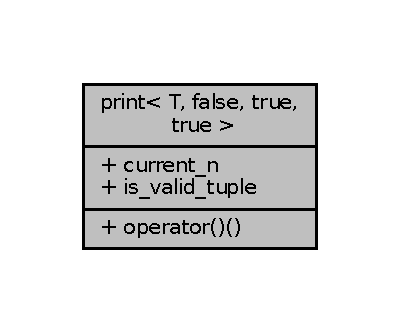
\includegraphics[width=192pt]{structprint_3_01T_00_01false_00_01true_00_01true_01_4__coll__graph}
\end{center}
\end{figure}
\subsection*{Public Types}
\begin{DoxyCompactItemize}
\item 
using \hyperlink{structprint_3_01T_00_01false_00_01true_00_01true_01_4_a2dae0d9d3db0a28ae73051bef2394aaa}{first\+\_\+element\+\_\+type} = typename std\+::tuple\+\_\+element\+\_\+t$<$ 0, T $>$
\item 
using \hyperlink{structprint_3_01T_00_01false_00_01true_00_01true_01_4_a6b6bfb81869a40026880ebd0d82cd25a}{n\+\_\+element\+\_\+type} = typename std\+::tuple\+\_\+element\+\_\+t$<$ std\+::tuple\+\_\+size$<$ T $>$()-\/1, T $>$
\end{DoxyCompactItemize}
\subsection*{Public Member Functions}
\begin{DoxyCompactItemize}
\item 
std\+::enable\+\_\+if\+\_\+t$<$ \hyperlink{structprint_3_01T_00_01false_00_01true_00_01true_01_4_ac26cb1e1f2d4e622fc9bd7ba97555dc4}{is\+\_\+valid\+\_\+tuple}, std\+::string $>$ \hyperlink{structprint_3_01T_00_01false_00_01true_00_01true_01_4_a6be8db822c3eb9a125d9f45eef7853a9}{operator()} (const T \&t)
\end{DoxyCompactItemize}
\subsection*{Static Public Attributes}
\begin{DoxyCompactItemize}
\item 
static constexpr size\+\_\+t \hyperlink{structprint_3_01T_00_01false_00_01true_00_01true_01_4_a1b88695798454d00772ed00dde4f10b8}{current\+\_\+n} = std\+::tuple\+\_\+size$<$T$>$() -\/ 1
\item 
static constexpr bool \hyperlink{structprint_3_01T_00_01false_00_01true_00_01true_01_4_ac26cb1e1f2d4e622fc9bd7ba97555dc4}{is\+\_\+valid\+\_\+tuple}
\end{DoxyCompactItemize}


\subsection{Member Typedef Documentation}
\index{print$<$ T, false, true, true $>$@{print$<$ T, false, true, true $>$}!first\+\_\+element\+\_\+type@{first\+\_\+element\+\_\+type}}
\index{first\+\_\+element\+\_\+type@{first\+\_\+element\+\_\+type}!print$<$ T, false, true, true $>$@{print$<$ T, false, true, true $>$}}
\subsubsection[{\texorpdfstring{first\+\_\+element\+\_\+type}{first_element_type}}]{\setlength{\rightskip}{0pt plus 5cm}template$<$typename T $>$ using {\bf print}$<$ T, false, true, true $>$\+::{\bf first\+\_\+element\+\_\+type} =  typename std\+::tuple\+\_\+element\+\_\+t$<$0,T$>$}\hypertarget{structprint_3_01T_00_01false_00_01true_00_01true_01_4_a2dae0d9d3db0a28ae73051bef2394aaa}{}\label{structprint_3_01T_00_01false_00_01true_00_01true_01_4_a2dae0d9d3db0a28ae73051bef2394aaa}
\index{print$<$ T, false, true, true $>$@{print$<$ T, false, true, true $>$}!n\+\_\+element\+\_\+type@{n\+\_\+element\+\_\+type}}
\index{n\+\_\+element\+\_\+type@{n\+\_\+element\+\_\+type}!print$<$ T, false, true, true $>$@{print$<$ T, false, true, true $>$}}
\subsubsection[{\texorpdfstring{n\+\_\+element\+\_\+type}{n_element_type}}]{\setlength{\rightskip}{0pt plus 5cm}template$<$typename T $>$ using {\bf print}$<$ T, false, true, true $>$\+::{\bf n\+\_\+element\+\_\+type} =  typename std\+::tuple\+\_\+element\+\_\+t$<$std\+::tuple\+\_\+size$<$T$>$()-\/1,T$>$}\hypertarget{structprint_3_01T_00_01false_00_01true_00_01true_01_4_a6b6bfb81869a40026880ebd0d82cd25a}{}\label{structprint_3_01T_00_01false_00_01true_00_01true_01_4_a6b6bfb81869a40026880ebd0d82cd25a}


\subsection{Member Function Documentation}
\index{print$<$ T, false, true, true $>$@{print$<$ T, false, true, true $>$}!operator()@{operator()}}
\index{operator()@{operator()}!print$<$ T, false, true, true $>$@{print$<$ T, false, true, true $>$}}
\subsubsection[{\texorpdfstring{operator()(const T \&t)}{operator()(const T &t)}}]{\setlength{\rightskip}{0pt plus 5cm}template$<$typename T $>$ std\+::enable\+\_\+if\+\_\+t$<${\bf is\+\_\+valid\+\_\+tuple}, std\+::string$>$ {\bf print}$<$ T, false, true, true $>$\+::operator() (
\begin{DoxyParamCaption}
\item[{const T \&}]{t}
\end{DoxyParamCaption}
)\hspace{0.3cm}{\ttfamily [inline]}}\hypertarget{structprint_3_01T_00_01false_00_01true_00_01true_01_4_a6be8db822c3eb9a125d9f45eef7853a9}{}\label{structprint_3_01T_00_01false_00_01true_00_01true_01_4_a6be8db822c3eb9a125d9f45eef7853a9}


Here is the call graph for this function\+:
\nopagebreak
\begin{figure}[H]
\begin{center}
\leavevmode
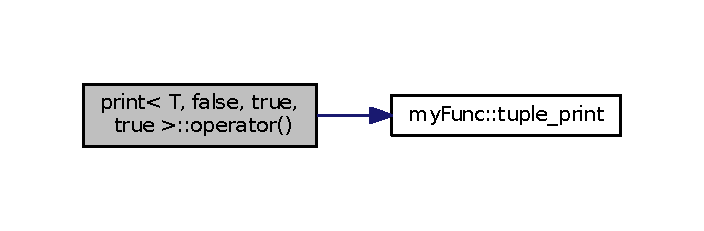
\includegraphics[width=338pt]{structprint_3_01T_00_01false_00_01true_00_01true_01_4_a6be8db822c3eb9a125d9f45eef7853a9_cgraph}
\end{center}
\end{figure}




\subsection{Member Data Documentation}
\index{print$<$ T, false, true, true $>$@{print$<$ T, false, true, true $>$}!current\+\_\+n@{current\+\_\+n}}
\index{current\+\_\+n@{current\+\_\+n}!print$<$ T, false, true, true $>$@{print$<$ T, false, true, true $>$}}
\subsubsection[{\texorpdfstring{current\+\_\+n}{current_n}}]{\setlength{\rightskip}{0pt plus 5cm}template$<$typename T $>$ constexpr size\+\_\+t {\bf print}$<$ T, false, true, true $>$\+::current\+\_\+n = std\+::tuple\+\_\+size$<$T$>$() -\/ 1\hspace{0.3cm}{\ttfamily [static]}}\hypertarget{structprint_3_01T_00_01false_00_01true_00_01true_01_4_a1b88695798454d00772ed00dde4f10b8}{}\label{structprint_3_01T_00_01false_00_01true_00_01true_01_4_a1b88695798454d00772ed00dde4f10b8}
\index{print$<$ T, false, true, true $>$@{print$<$ T, false, true, true $>$}!is\+\_\+valid\+\_\+tuple@{is\+\_\+valid\+\_\+tuple}}
\index{is\+\_\+valid\+\_\+tuple@{is\+\_\+valid\+\_\+tuple}!print$<$ T, false, true, true $>$@{print$<$ T, false, true, true $>$}}
\subsubsection[{\texorpdfstring{is\+\_\+valid\+\_\+tuple}{is_valid_tuple}}]{\setlength{\rightskip}{0pt plus 5cm}template$<$typename T $>$ constexpr bool {\bf print}$<$ T, false, true, true $>$\+::is\+\_\+valid\+\_\+tuple\hspace{0.3cm}{\ttfamily [static]}}\hypertarget{structprint_3_01T_00_01false_00_01true_00_01true_01_4_ac26cb1e1f2d4e622fc9bd7ba97555dc4}{}\label{structprint_3_01T_00_01false_00_01true_00_01true_01_4_ac26cb1e1f2d4e622fc9bd7ba97555dc4}
{\bfseries Initial value\+:}
\begin{DoxyCode}
= \hyperlink{namespacemyFunc_aa757a804546f113b7cadf75b0a1ec7e1}{myFunc::is\_one\_of\_v}<
            \hyperlink{structprint_3_01T_00_01false_00_01true_00_01true_01_4_a2dae0d9d3db0a28ae73051bef2394aaa}{first\_element\_type},
            \hyperlink{structprint_3_01T_00_01false_00_01true_00_01true_01_4_a6b6bfb81869a40026880ebd0d82cd25a}{n\_element\_type},
            \hyperlink{structprint_3_01T_00_01false_00_01true_00_01true_01_4_a1b88695798454d00772ed00dde4f10b8}{current\_n},
            T>
\end{DoxyCode}


The documentation for this struct was generated from the following file\+:\begin{DoxyCompactItemize}
\item 
\hyperlink{print__ip_8cpp}{print\+\_\+ip.\+cpp}\end{DoxyCompactItemize}

\hypertarget{structprint_3_01T_00_01true_00_01false_00_01false_01_4}{}\section{print$<$ T, true, false, false $>$ Struct Template Reference}
\label{structprint_3_01T_00_01true_00_01false_00_01false_01_4}\index{print$<$ T, true, false, false $>$@{print$<$ T, true, false, false $>$}}
\subsection*{Public Member Functions}
\begin{DoxyCompactItemize}
\item 
std\+::string \hyperlink{structprint_3_01T_00_01true_00_01false_00_01false_01_4_a441334718f623594d87bff6576ffeb56}{operator()} (T t)
\end{DoxyCompactItemize}


\subsection{Member Function Documentation}
\index{print$<$ T, true, false, false $>$@{print$<$ T, true, false, false $>$}!operator()@{operator()}}
\index{operator()@{operator()}!print$<$ T, true, false, false $>$@{print$<$ T, true, false, false $>$}}
\subsubsection[{\texorpdfstring{operator()(\+T t)}{operator()(T t)}}]{\setlength{\rightskip}{0pt plus 5cm}template$<$typename T $>$ std\+::string {\bf print}$<$ T, true, false, false $>$\+::operator() (
\begin{DoxyParamCaption}
\item[{T}]{t}
\end{DoxyParamCaption}
)\hspace{0.3cm}{\ttfamily [inline]}}\hypertarget{structprint_3_01T_00_01true_00_01false_00_01false_01_4_a441334718f623594d87bff6576ffeb56}{}\label{structprint_3_01T_00_01true_00_01false_00_01false_01_4_a441334718f623594d87bff6576ffeb56}


The documentation for this struct was generated from the following file\+:\begin{DoxyCompactItemize}
\item 
\hyperlink{print__ip_8cpp}{print\+\_\+ip.\+cpp}\end{DoxyCompactItemize}

\hypertarget{structmyFunc_1_1TuplePrinter}{}\section{my\+Func\+:\+:Tuple\+Printer$<$ Tuple, N $>$ Struct Template Reference}
\label{structmyFunc_1_1TuplePrinter}\index{my\+Func\+::\+Tuple\+Printer$<$ Tuple, N $>$@{my\+Func\+::\+Tuple\+Printer$<$ Tuple, N $>$}}


Collaboration diagram for my\+Func\+:\+:Tuple\+Printer$<$ Tuple, N $>$\+:
\nopagebreak
\begin{figure}[H]
\begin{center}
\leavevmode
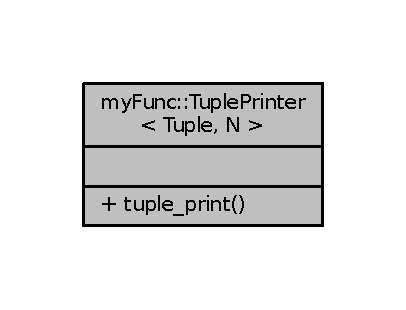
\includegraphics[width=195pt]{structmyFunc_1_1TuplePrinter__coll__graph}
\end{center}
\end{figure}
\subsection*{Static Public Member Functions}
\begin{DoxyCompactItemize}
\item 
static void \hyperlink{structmyFunc_1_1TuplePrinter_ac5e1b24bcfeb6b1f482babfc35eec03d}{tuple\+\_\+print} (const Tuple \&t)
\end{DoxyCompactItemize}


\subsection{Member Function Documentation}
\index{my\+Func\+::\+Tuple\+Printer@{my\+Func\+::\+Tuple\+Printer}!tuple\+\_\+print@{tuple\+\_\+print}}
\index{tuple\+\_\+print@{tuple\+\_\+print}!my\+Func\+::\+Tuple\+Printer@{my\+Func\+::\+Tuple\+Printer}}
\subsubsection[{\texorpdfstring{tuple\+\_\+print(const Tuple \&t)}{tuple_print(const Tuple &t)}}]{\setlength{\rightskip}{0pt plus 5cm}template$<$class Tuple , std\+::size\+\_\+t N$>$ static void {\bf my\+Func\+::\+Tuple\+Printer}$<$ Tuple, N $>$\+::tuple\+\_\+print (
\begin{DoxyParamCaption}
\item[{const Tuple \&}]{t}
\end{DoxyParamCaption}
)\hspace{0.3cm}{\ttfamily [inline]}, {\ttfamily [static]}}\hypertarget{structmyFunc_1_1TuplePrinter_ac5e1b24bcfeb6b1f482babfc35eec03d}{}\label{structmyFunc_1_1TuplePrinter_ac5e1b24bcfeb6b1f482babfc35eec03d}


The documentation for this struct was generated from the following file\+:\begin{DoxyCompactItemize}
\item 
\hyperlink{print__ip_8cpp}{print\+\_\+ip.\+cpp}\end{DoxyCompactItemize}

\hypertarget{structmyFunc_1_1TuplePrinter_3_01Tuple_00_011_01_4}{}\section{my\+Func\+:\+:Tuple\+Printer$<$ Tuple, 1 $>$ Struct Template Reference}
\label{structmyFunc_1_1TuplePrinter_3_01Tuple_00_011_01_4}\index{my\+Func\+::\+Tuple\+Printer$<$ Tuple, 1 $>$@{my\+Func\+::\+Tuple\+Printer$<$ Tuple, 1 $>$}}
\subsection*{Static Public Member Functions}
\begin{DoxyCompactItemize}
\item 
static void \hyperlink{structmyFunc_1_1TuplePrinter_3_01Tuple_00_011_01_4_ade88d5a9d8393a74646cf0f44cac2294}{tuple\+\_\+print} (const Tuple \&t)
\end{DoxyCompactItemize}


\subsection{Member Function Documentation}
\index{my\+Func\+::\+Tuple\+Printer$<$ Tuple, 1 $>$@{my\+Func\+::\+Tuple\+Printer$<$ Tuple, 1 $>$}!tuple\+\_\+print@{tuple\+\_\+print}}
\index{tuple\+\_\+print@{tuple\+\_\+print}!my\+Func\+::\+Tuple\+Printer$<$ Tuple, 1 $>$@{my\+Func\+::\+Tuple\+Printer$<$ Tuple, 1 $>$}}
\subsubsection[{\texorpdfstring{tuple\+\_\+print(const Tuple \&t)}{tuple_print(const Tuple &t)}}]{\setlength{\rightskip}{0pt plus 5cm}template$<$class Tuple $>$ static void {\bf my\+Func\+::\+Tuple\+Printer}$<$ Tuple, 1 $>$\+::tuple\+\_\+print (
\begin{DoxyParamCaption}
\item[{const Tuple \&}]{t}
\end{DoxyParamCaption}
)\hspace{0.3cm}{\ttfamily [inline]}, {\ttfamily [static]}}\hypertarget{structmyFunc_1_1TuplePrinter_3_01Tuple_00_011_01_4_ade88d5a9d8393a74646cf0f44cac2294}{}\label{structmyFunc_1_1TuplePrinter_3_01Tuple_00_011_01_4_ade88d5a9d8393a74646cf0f44cac2294}


The documentation for this struct was generated from the following file\+:\begin{DoxyCompactItemize}
\item 
\hyperlink{print__ip_8cpp}{print\+\_\+ip.\+cpp}\end{DoxyCompactItemize}

\chapter{File Documentation}
\hypertarget{CMakeLists_8txt}{}\section{C\+Make\+Lists.\+txt File Reference}
\label{CMakeLists_8txt}\index{C\+Make\+Lists.\+txt@{C\+Make\+Lists.\+txt}}
\subsection*{Functions}
\begin{DoxyCompactItemize}
\item 
\hyperlink{CMakeLists_8txt_a149ac2a2c7b91844a3e1b08ae0d9ed3f}{cmake\+\_\+minimum\+\_\+required} (V\+E\+R\+S\+I\+ON 3.\+2) project(print\+\_\+ip V\+E\+R\+S\+I\+ON 0.\+0.\$E\+NV
\item 
\hyperlink{CMakeLists_8txt_a0d34b2a0dad72d0f6e9b3498ff841cf1}{find\+\_\+package} (Boost C\+O\+M\+P\+O\+N\+E\+N\+TS unit\+\_\+test\+\_\+framework R\+E\+Q\+U\+I\+R\+ED) add\+\_\+executable(print\+\_\+ip main.\+cpp) add\+\_\+library(ip\+\_\+lib print\+\_\+ip.\+cpp) add\+\_\+executable(test\+\_\+ip\+\_\+print test\+\_\+ip\+\_\+print.\+cpp) \hyperlink{CMakeLists_8txt_a981e44eb2eb86a763ac0609e8597a611}{set\+\_\+target\+\_\+properties}(print\+\_\+ip ip\+\_\+lib test\+\_\+ip\+\_\+print P\+R\+O\+P\+E\+R\+T\+I\+ES C\+X\+X\+\_\+\+S\+T\+A\+N\+D\+A\+RD 14 C\+X\+X\+\_\+\+S\+T\+A\+N\+D\+A\+R\+D\+\_\+\+R\+E\+Q\+U\+I\+R\+ED ON C\+O\+M\+P\+I\+L\+E\+\_\+\+O\+P\+T\+I\+O\+NS\char`\"{}-\/Wpedantic
\item 
Wextra \hyperlink{CMakeLists_8txt_a981e44eb2eb86a763ac0609e8597a611}{set\+\_\+target\+\_\+properties} (test\+\_\+ip\+\_\+print P\+R\+O\+P\+E\+R\+T\+I\+ES C\+O\+M\+P\+I\+L\+E\+\_\+\+D\+E\+F\+I\+N\+I\+T\+I\+O\+NS B\+O\+O\+S\+T\+\_\+\+T\+E\+S\+T\+\_\+\+D\+Y\+N\+\_\+\+L\+I\+NK I\+N\+C\+L\+U\+D\+E\+\_\+\+D\+I\+R\+E\+C\+T\+O\+R\+I\+ES \$\{Boost\+\_\+\+I\+N\+C\+L\+U\+D\+E\+\_\+\+D\+IR\}) target\+\_\+link\+\_\+libraries(print\+\_\+ip ip\+\_\+lib) target\+\_\+link\+\_\+libraries(test\+\_\+ip\+\_\+print \$
\item 
ip\+\_\+lib \hyperlink{CMakeLists_8txt_ad5b09882d4ffa0b2549cdcd18161c85d}{install} (T\+A\+R\+G\+E\+TS print\+\_\+ip R\+U\+N\+T\+I\+ME D\+E\+S\+T\+I\+N\+A\+T\+I\+ON bin) \hyperlink{CMakeLists_8txt_abed8177b0359bb37e78aebe0412cc156}{set}(C\+P\+A\+C\+K\+\_\+\+G\+E\+N\+E\+R\+A\+T\+OR D\+EB) \hyperlink{CMakeLists_8txt_abed8177b0359bb37e78aebe0412cc156}{set}(C\+P\+A\+C\+K\+\_\+\+P\+A\+C\+K\+A\+G\+E\+\_\+\+V\+E\+R\+S\+I\+O\+N\+\_\+\+M\+A\+J\+OR\char`\"{}\$
\item 
\hyperlink{CMakeLists_8txt_abed8177b0359bb37e78aebe0412cc156}{set} (C\+P\+A\+C\+K\+\_\+\+P\+A\+C\+K\+A\+G\+E\+\_\+\+V\+E\+R\+S\+I\+O\+N\+\_\+\+M\+I\+N\+OR\char`\"{}\$\{P\+R\+O\+J\+E\+C\+T\+\_\+\+V\+E\+R\+S\+I\+O\+N\+\_\+\+M\+I\+N\+OR\}\char`\"{}) set(C\+P\+A\+C\+K\+\_\+\+P\+A\+C\+K\+A\+G\+E\+\_\+\+V\+E\+R\+S\+I\+O\+N\+\_\+\+P\+A\+T\+CH\char`\"{}\$
\end{DoxyCompactItemize}
\subsection*{Variables}
\begin{DoxyCompactItemize}
\item 
\hyperlink{CMakeLists_8txt_ad4f6886266572e51d198a61a6c762ce5}{Wall}
\end{DoxyCompactItemize}


\subsection{Function Documentation}
\index{C\+Make\+Lists.\+txt@{C\+Make\+Lists.\+txt}!cmake\+\_\+minimum\+\_\+required@{cmake\+\_\+minimum\+\_\+required}}
\index{cmake\+\_\+minimum\+\_\+required@{cmake\+\_\+minimum\+\_\+required}!C\+Make\+Lists.\+txt@{C\+Make\+Lists.\+txt}}
\subsubsection[{\texorpdfstring{cmake\+\_\+minimum\+\_\+required(\+V\+E\+R\+S\+I\+O\+N 3.\+2) project(print\+\_\+ip V\+E\+R\+S\+I\+O\+N 0.\+0.\$\+E\+NV}{cmake_minimum_required(VERSION 3.2) project(print_ip VERSION 0.0.$ENV}}]{\setlength{\rightskip}{0pt plus 5cm}cmake\+\_\+minimum\+\_\+required (
\begin{DoxyParamCaption}
\item[{V\+E\+R\+S\+I\+ON 3.}]{2}
\end{DoxyParamCaption}
)}\hypertarget{CMakeLists_8txt_a149ac2a2c7b91844a3e1b08ae0d9ed3f}{}\label{CMakeLists_8txt_a149ac2a2c7b91844a3e1b08ae0d9ed3f}


Here is the call graph for this function\+:
\nopagebreak
\begin{figure}[H]
\begin{center}
\leavevmode
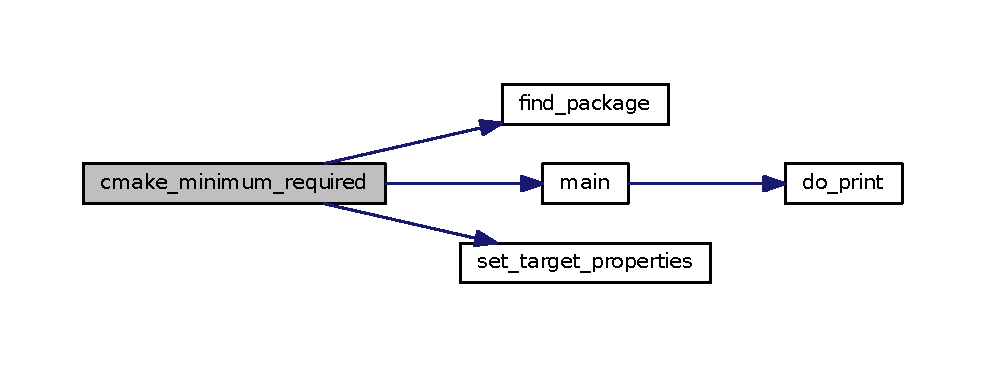
\includegraphics[width=350pt]{CMakeLists_8txt_a149ac2a2c7b91844a3e1b08ae0d9ed3f_cgraph}
\end{center}
\end{figure}


\index{C\+Make\+Lists.\+txt@{C\+Make\+Lists.\+txt}!find\+\_\+package@{find\+\_\+package}}
\index{find\+\_\+package@{find\+\_\+package}!C\+Make\+Lists.\+txt@{C\+Make\+Lists.\+txt}}
\subsubsection[{\texorpdfstring{find\+\_\+package(\+Boost C\+O\+M\+P\+O\+N\+E\+N\+T\+S unit\+\_\+test\+\_\+framework R\+E\+Q\+U\+I\+R\+E\+D) add\+\_\+executable(print\+\_\+ip main.\+cpp) add\+\_\+library(ip\+\_\+lib print\+\_\+ip.\+cpp) add\+\_\+executable(test\+\_\+ip\+\_\+print test\+\_\+ip\+\_\+print.\+cpp) set\+\_\+target\+\_\+properties(print\+\_\+ip ip\+\_\+lib test\+\_\+ip\+\_\+print P\+R\+O\+P\+E\+R\+T\+I\+E\+S C\+X\+X\+\_\+\+S\+T\+A\+N\+D\+A\+R\+D 14 C\+X\+X\+\_\+\+S\+T\+A\+N\+D\+A\+R\+D\+\_\+\+R\+E\+Q\+U\+I\+R\+E\+D O\+N C\+O\+M\+P\+I\+L\+E\+\_\+\+O\+P\+T\+I\+O\+NS""-\/\+Wpedantic}{find_package(Boost COMPONENTS unit_test_framework REQUIRED) add_executable(print_ip main.cpp) add_library(ip_lib print_ip.cpp) add_executable(test_ip_print test_ip_print.cpp) set_target_properties(print_ip ip_lib test_ip_print PROPERTIES CXX_STANDARD 14 CXX_STANDARD_REQUIRED ON COMPILE_OPTIONS"-Wpedantic}}]{\setlength{\rightskip}{0pt plus 5cm}find\+\_\+package (
\begin{DoxyParamCaption}
\item[{Boost C\+O\+M\+P\+O\+N\+E\+N\+TS unit\+\_\+test\+\_\+framework}]{R\+E\+Q\+U\+I\+R\+ED}
\end{DoxyParamCaption}
)}\hypertarget{CMakeLists_8txt_a0d34b2a0dad72d0f6e9b3498ff841cf1}{}\label{CMakeLists_8txt_a0d34b2a0dad72d0f6e9b3498ff841cf1}


Here is the caller graph for this function\+:
\nopagebreak
\begin{figure}[H]
\begin{center}
\leavevmode
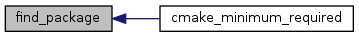
\includegraphics[width=341pt]{CMakeLists_8txt_a0d34b2a0dad72d0f6e9b3498ff841cf1_icgraph}
\end{center}
\end{figure}


\index{C\+Make\+Lists.\+txt@{C\+Make\+Lists.\+txt}!install@{install}}
\index{install@{install}!C\+Make\+Lists.\+txt@{C\+Make\+Lists.\+txt}}
\subsubsection[{\texorpdfstring{install(\+T\+A\+R\+G\+E\+T\+S print\+\_\+ip R\+U\+N\+T\+I\+M\+E D\+E\+S\+T\+I\+N\+A\+T\+I\+O\+N bin) set(\+C\+P\+A\+C\+K\+\_\+\+G\+E\+N\+E\+R\+A\+T\+O\+R D\+E\+B) set(\+C\+P\+A\+C\+K\+\_\+\+P\+A\+C\+K\+A\+G\+E\+\_\+\+V\+E\+R\+S\+I\+O\+N\+\_\+\+M\+A\+J\+OR""\$}{install(TARGETS print_ip RUNTIME DESTINATION bin) set(CPACK_GENERATOR DEB) set(CPACK_PACKAGE_VERSION_MAJOR"$}}]{\setlength{\rightskip}{0pt plus 5cm}ip\+\_\+lib install (
\begin{DoxyParamCaption}
\item[{T\+A\+R\+G\+E\+TS print\+\_\+ip R\+U\+N\+T\+I\+ME D\+E\+S\+T\+I\+N\+A\+T\+I\+ON}]{bin}
\end{DoxyParamCaption}
)}\hypertarget{CMakeLists_8txt_ad5b09882d4ffa0b2549cdcd18161c85d}{}\label{CMakeLists_8txt_ad5b09882d4ffa0b2549cdcd18161c85d}
\index{C\+Make\+Lists.\+txt@{C\+Make\+Lists.\+txt}!set@{set}}
\index{set@{set}!C\+Make\+Lists.\+txt@{C\+Make\+Lists.\+txt}}
\subsubsection[{\texorpdfstring{set(\+C\+P\+A\+C\+K\+\_\+\+P\+A\+C\+K\+A\+G\+E\+\_\+\+V\+E\+R\+S\+I\+O\+N\+\_\+\+M\+I\+N\+OR""\$\lcurly{}P\+R\+O\+J\+E\+C\+T\+\_\+\+V\+E\+R\+S\+I\+O\+N\+\_\+\+M\+I\+N\+OR\rcurly{}"") set(\+C\+P\+A\+C\+K\+\_\+\+P\+A\+C\+K\+A\+G\+E\+\_\+\+V\+E\+R\+S\+I\+O\+N\+\_\+\+P\+A\+T\+CH""\$}{set(CPACK_PACKAGE_VERSION_MINOR"$\{PROJECT_VERSION_MINOR\}") set(CPACK_PACKAGE_VERSION_PATCH"$}}]{\setlength{\rightskip}{0pt plus 5cm}set (
\begin{DoxyParamCaption}
\item[{C\+P\+A\+C\+K\+\_\+\+P\+A\+C\+K\+A\+G\+E\+\_\+\+V\+E\+R\+S\+I\+O\+N\+\_\+\+M\+I\+N\+OR\char`\"{}\$\{P\+R\+O\+J\+E\+C\+T\+\_\+\+V\+E\+R\+S\+I\+O\+N\+\_\+\+M\+I\+N\+OR\}\char`\"{}}]{}
\end{DoxyParamCaption}
)}\hypertarget{CMakeLists_8txt_abed8177b0359bb37e78aebe0412cc156}{}\label{CMakeLists_8txt_abed8177b0359bb37e78aebe0412cc156}
\index{C\+Make\+Lists.\+txt@{C\+Make\+Lists.\+txt}!set\+\_\+target\+\_\+properties@{set\+\_\+target\+\_\+properties}}
\index{set\+\_\+target\+\_\+properties@{set\+\_\+target\+\_\+properties}!C\+Make\+Lists.\+txt@{C\+Make\+Lists.\+txt}}
\subsubsection[{\texorpdfstring{set\+\_\+target\+\_\+properties(test\+\_\+ip\+\_\+print P\+R\+O\+P\+E\+R\+T\+I\+E\+S C\+O\+M\+P\+I\+L\+E\+\_\+\+D\+E\+F\+I\+N\+I\+T\+I\+O\+N\+S B\+O\+O\+S\+T\+\_\+\+T\+E\+S\+T\+\_\+\+D\+Y\+N\+\_\+\+L\+I\+N\+K I\+N\+C\+L\+U\+D\+E\+\_\+\+D\+I\+R\+E\+C\+T\+O\+R\+I\+E\+S \$\lcurly{}Boost\+\_\+\+I\+N\+C\+L\+U\+D\+E\+\_\+\+D\+IR\rcurly{}) target\+\_\+link\+\_\+libraries(print\+\_\+ip ip\+\_\+lib) target\+\_\+link\+\_\+libraries(test\+\_\+ip\+\_\+print \$}{set_target_properties(test_ip_print PROPERTIES COMPILE_DEFINITIONS BOOST_TEST_DYN_LINK INCLUDE_DIRECTORIES $\{Boost_INCLUDE_DIR\}) target_link_libraries(print_ip ip_lib) target_link_libraries(test_ip_print $}}]{\setlength{\rightskip}{0pt plus 5cm}Wextra set\+\_\+target\+\_\+properties (
\begin{DoxyParamCaption}
\item[{test\+\_\+ip\+\_\+print P\+R\+O\+P\+E\+R\+T\+I\+ES C\+O\+M\+P\+I\+L\+E\+\_\+\+D\+E\+F\+I\+N\+I\+T\+I\+O\+NS B\+O\+O\+S\+T\+\_\+\+T\+E\+S\+T\+\_\+\+D\+Y\+N\+\_\+\+L\+I\+NK I\+N\+C\+L\+U\+D\+E\+\_\+\+D\+I\+R\+E\+C\+T\+O\+R\+I\+ES \$\{Boost\+\_\+\+I\+N\+C\+L\+U\+D\+E\+\_\+\+D\+IR\}}]{}
\end{DoxyParamCaption}
)}\hypertarget{CMakeLists_8txt_a981e44eb2eb86a763ac0609e8597a611}{}\label{CMakeLists_8txt_a981e44eb2eb86a763ac0609e8597a611}


Here is the caller graph for this function\+:
\nopagebreak
\begin{figure}[H]
\begin{center}
\leavevmode
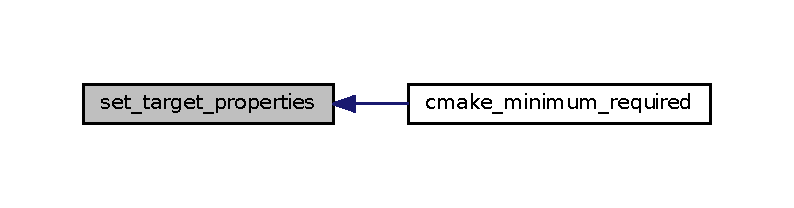
\includegraphics[width=350pt]{CMakeLists_8txt_a981e44eb2eb86a763ac0609e8597a611_icgraph}
\end{center}
\end{figure}




\subsection{Variable Documentation}
\index{C\+Make\+Lists.\+txt@{C\+Make\+Lists.\+txt}!Wall@{Wall}}
\index{Wall@{Wall}!C\+Make\+Lists.\+txt@{C\+Make\+Lists.\+txt}}
\subsubsection[{\texorpdfstring{Wall}{Wall}}]{\setlength{\rightskip}{0pt plus 5cm}Wall}\hypertarget{CMakeLists_8txt_ad4f6886266572e51d198a61a6c762ce5}{}\label{CMakeLists_8txt_ad4f6886266572e51d198a61a6c762ce5}

\hypertarget{main_8cpp}{}\section{main.\+cpp File Reference}
\label{main_8cpp}\index{main.\+cpp@{main.\+cpp}}
{\ttfamily \#include $<$vector$>$}\\*
{\ttfamily \#include $<$list$>$}\\*
{\ttfamily \#include \char`\"{}print\+\_\+ip.\+cpp\char`\"{}}\\*
Include dependency graph for main.\+cpp\+:
\nopagebreak
\begin{figure}[H]
\begin{center}
\leavevmode
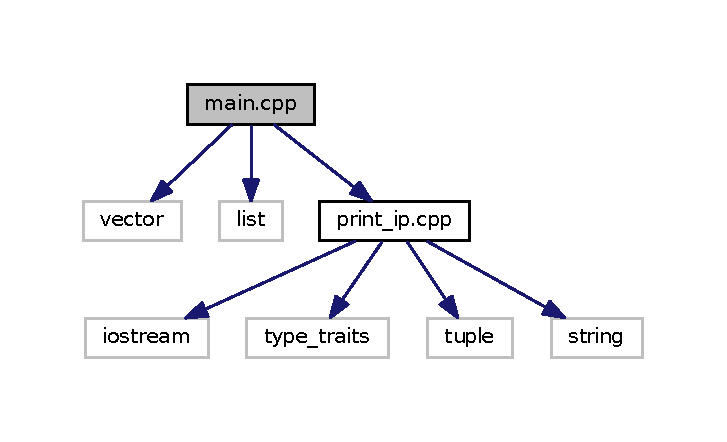
\includegraphics[width=349pt]{main_8cpp__incl}
\end{center}
\end{figure}
\subsection*{Functions}
\begin{DoxyCompactItemize}
\item 
int \hyperlink{main_8cpp_ae66f6b31b5ad750f1fe042a706a4e3d4}{main} ()
\end{DoxyCompactItemize}


\subsection{Function Documentation}
\index{main.\+cpp@{main.\+cpp}!main@{main}}
\index{main@{main}!main.\+cpp@{main.\+cpp}}
\subsubsection[{\texorpdfstring{main()}{main()}}]{\setlength{\rightskip}{0pt plus 5cm}int main (
\begin{DoxyParamCaption}
{}
\end{DoxyParamCaption}
)}\hypertarget{main_8cpp_ae66f6b31b5ad750f1fe042a706a4e3d4}{}\label{main_8cpp_ae66f6b31b5ad750f1fe042a706a4e3d4}

\hypertarget{print__ip_8cpp}{}\section{print\+\_\+ip.\+cpp File Reference}
\label{print__ip_8cpp}\index{print\+\_\+ip.\+cpp@{print\+\_\+ip.\+cpp}}
{\ttfamily \#include $<$iostream$>$}\\*
{\ttfamily \#include $<$type\+\_\+traits$>$}\\*
{\ttfamily \#include $<$tuple$>$}\\*
{\ttfamily \#include $<$string$>$}\\*
Include dependency graph for print\+\_\+ip.\+cpp\+:
\nopagebreak
\begin{figure}[H]
\begin{center}
\leavevmode
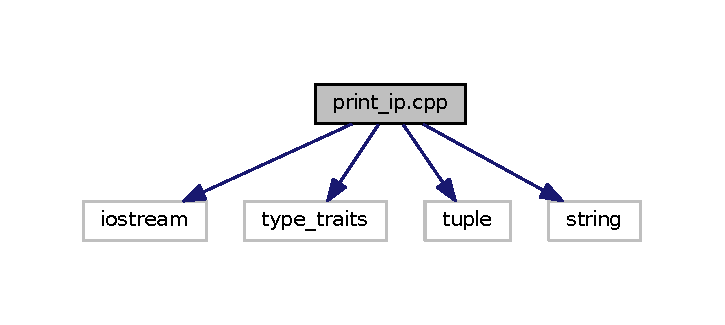
\includegraphics[width=348pt]{print__ip_8cpp__incl}
\end{center}
\end{figure}
This graph shows which files directly or indirectly include this file\+:
\nopagebreak
\begin{figure}[H]
\begin{center}
\leavevmode
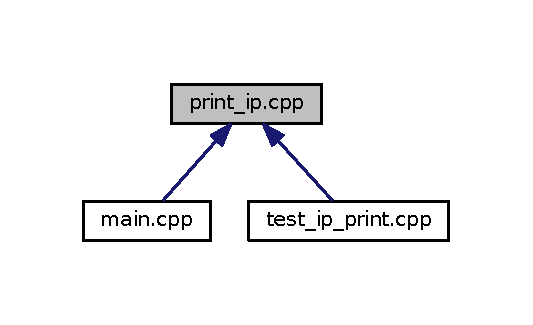
\includegraphics[width=256pt]{print__ip_8cpp__dep__incl}
\end{center}
\end{figure}
\subsection*{Classes}
\begin{DoxyCompactItemize}
\item 
struct \hyperlink{structmyFunc_1_1IsTupleImpl}{my\+Func\+::\+Is\+Tuple\+Impl$<$ T $>$}
\item 
struct \hyperlink{structmyFunc_1_1IsTupleImpl_3_01std_1_1tuple_3_01U_8_8_8_01_4_01_4}{my\+Func\+::\+Is\+Tuple\+Impl$<$ std\+::tuple$<$ U... $>$ $>$}
\item 
struct \hyperlink{structmyFunc_1_1is__one__of}{my\+Func\+::is\+\_\+one\+\_\+of$<$ T, U, i, V $>$}
\item 
struct \hyperlink{structmyFunc_1_1is__one__of_3_01T_00_01T_00_011_00_01V_01_4}{my\+Func\+::is\+\_\+one\+\_\+of$<$ T, T, 1, V $>$}
\item 
struct \hyperlink{structmyFunc_1_1is__one__of_3_01T_00_01T_00_01i_00_01V_01_4}{my\+Func\+::is\+\_\+one\+\_\+of$<$ T, T, i, V $>$}
\item 
struct \hyperlink{structmyFunc_1_1TuplePrinter}{my\+Func\+::\+Tuple\+Printer$<$ Tuple, N $>$}
\item 
struct \hyperlink{structmyFunc_1_1TuplePrinter_3_01Tuple_00_011_01_4}{my\+Func\+::\+Tuple\+Printer$<$ Tuple, 1 $>$}
\item 
struct \hyperlink{structprint}{print$<$ T, is\+\_\+integral, is\+\_\+object, is\+\_\+tuple $>$}
\item 
union \hyperlink{unionbyteview}{byteview$<$ T $>$}
\item 
struct \hyperlink{structprint_3_01T_00_01true_00_01false_00_01false_01_4}{print$<$ T, true, false, false $>$}
\item 
struct \hyperlink{structprint_3_01T_00_01false_00_01true_00_01false_01_4}{print$<$ T, false, true, false $>$}
\item 
struct \hyperlink{structprint_3_01T_00_01false_00_01true_00_01true_01_4}{print$<$ T, false, true, true $>$}
\end{DoxyCompactItemize}
\subsection*{Namespaces}
\begin{DoxyCompactItemize}
\item 
 \hyperlink{namespacestd}{std}
\item 
 \hyperlink{namespacemyFunc}{my\+Func}
\end{DoxyCompactItemize}
\subsection*{Functions}
\begin{DoxyCompactItemize}
\item 
{\footnotesize template$<$typename T $>$ }\\constexpr bool \hyperlink{namespacemyFunc_afe24a25839d94fd3368128576589722a}{my\+Func\+::is\+\_\+tuple\+\_\+v} ()
\item 
{\footnotesize template$<$typename T $>$ }\\std\+::enable\+\_\+if\+\_\+t$<$ \hyperlink{namespacestd_ae1e905cdb2694181466fae8f8dd8f8e8}{std\+::is\+\_\+compound\+\_\+v}$<$ T $>$, std\+::string $>$ \hyperlink{namespacemyFunc_a2880ec2f77273fe6723e3a9bf280f8f4}{my\+Func\+::all\+\_\+to\+\_\+sting} (T t)
\item 
{\footnotesize template$<$typename T $>$ }\\std\+::enable\+\_\+if\+\_\+t$<$ \hyperlink{namespacestd_a824c5eb1a7e8aafa382dc9af3329a9e8}{std\+::is\+\_\+integral\+\_\+v}$<$ T $>$, std\+::string $>$ \hyperlink{namespacemyFunc_a501f8e9903912dcbd57e865a214c6568}{my\+Func\+::all\+\_\+to\+\_\+sting} (T t)
\item 
{\footnotesize template$<$class... Args$>$ }\\void \hyperlink{namespacemyFunc_a6588b7e742bf09aefea7d531f5c8ca6e}{my\+Func\+::tuple\+\_\+print} (const std\+::tuple$<$ Args... $>$ \&t)
\item 
{\footnotesize template$<$typename T $>$ }\\std\+::string \hyperlink{print__ip_8cpp_adb9c8fb50d681b29329c3859d6a2e2db}{do\+\_\+print} (const T \&t)
\end{DoxyCompactItemize}
\subsection*{Variables}
\begin{DoxyCompactItemize}
\item 
{\footnotesize template$<$typename T $>$ }\\constexpr bool \hyperlink{namespacestd_a824c5eb1a7e8aafa382dc9af3329a9e8}{std\+::is\+\_\+integral\+\_\+v} = is\+\_\+integral$<$T$>$\+::value
\item 
{\footnotesize template$<$typename T $>$ }\\constexpr bool \hyperlink{namespacestd_ae1e905cdb2694181466fae8f8dd8f8e8}{std\+::is\+\_\+compound\+\_\+v} = is\+\_\+compound$<$T$>$\+::value
\item 
{\footnotesize template$<$typename T , typename U , size\+\_\+t i, typename V $>$ }\\constexpr bool \hyperlink{namespacemyFunc_aa757a804546f113b7cadf75b0a1ec7e1}{my\+Func\+::is\+\_\+one\+\_\+of\+\_\+v} = is\+\_\+one\+\_\+of$<$T, U, i, V$>$\+::value
\end{DoxyCompactItemize}


\subsection{Function Documentation}
\index{print\+\_\+ip.\+cpp@{print\+\_\+ip.\+cpp}!do\+\_\+print@{do\+\_\+print}}
\index{do\+\_\+print@{do\+\_\+print}!print\+\_\+ip.\+cpp@{print\+\_\+ip.\+cpp}}
\subsubsection[{\texorpdfstring{do\+\_\+print(const T \&t)}{do_print(const T &t)}}]{\setlength{\rightskip}{0pt plus 5cm}template$<$typename T $>$ std\+::string do\+\_\+print (
\begin{DoxyParamCaption}
\item[{const T \&}]{t}
\end{DoxyParamCaption}
)}\hypertarget{print__ip_8cpp_adb9c8fb50d681b29329c3859d6a2e2db}{}\label{print__ip_8cpp_adb9c8fb50d681b29329c3859d6a2e2db}

\hypertarget{test__ip__print_8cpp}{}\section{test\+\_\+ip\+\_\+print.\+cpp File Reference}
\label{test__ip__print_8cpp}\index{test\+\_\+ip\+\_\+print.\+cpp@{test\+\_\+ip\+\_\+print.\+cpp}}
{\ttfamily \#include $<$boost/test/unit\+\_\+test.\+hpp$>$}\\*
{\ttfamily \#include \char`\"{}print\+\_\+ip.\+cpp\char`\"{}}\\*
Include dependency graph for test\+\_\+ip\+\_\+print.\+cpp\+:
\nopagebreak
\begin{figure}[H]
\begin{center}
\leavevmode
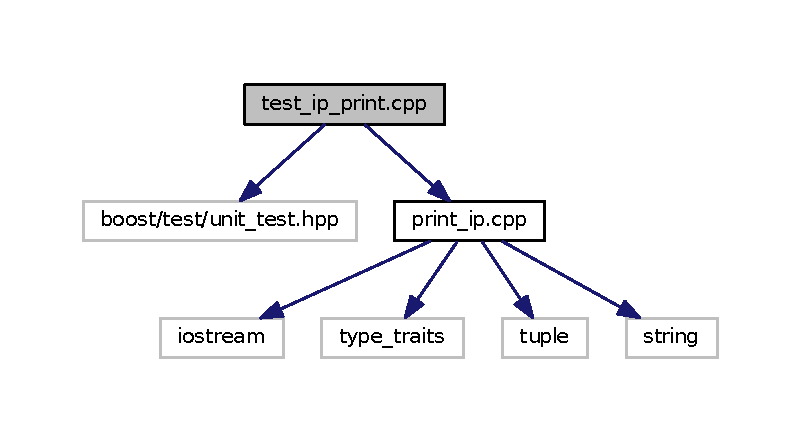
\includegraphics[width=350pt]{test__ip__print_8cpp__incl}
\end{center}
\end{figure}
\subsection*{Macros}
\begin{DoxyCompactItemize}
\item 
\#define \hyperlink{test__ip__print_8cpp_a6b2a3852db8bb19ab6909bac01859985}{B\+O\+O\+S\+T\+\_\+\+T\+E\+S\+T\+\_\+\+M\+O\+D\+U\+LE}~test\+\_\+module
\end{DoxyCompactItemize}
\subsection*{Functions}
\begin{DoxyCompactItemize}
\item 
\hyperlink{test__ip__print_8cpp_ab85b737b15d7ec91dd3b82af8d296f40}{B\+O\+O\+S\+T\+\_\+\+A\+U\+T\+O\+\_\+\+T\+E\+S\+T\+\_\+\+C\+A\+SE} (print\+\_\+test\+\_\+0)
\item 
\hyperlink{test__ip__print_8cpp_a8ca48550418bc3eaeacd892f6f311f53}{B\+O\+O\+S\+T\+\_\+\+A\+U\+T\+O\+\_\+\+T\+E\+S\+T\+\_\+\+C\+A\+SE} (print\+\_\+test\+\_\+1)
\item 
\hyperlink{test__ip__print_8cpp_aea4481282587bde1a22312b47799faf1}{B\+O\+O\+S\+T\+\_\+\+A\+U\+T\+O\+\_\+\+T\+E\+S\+T\+\_\+\+C\+A\+SE} (print\+\_\+test\+\_\+2)
\item 
\hyperlink{test__ip__print_8cpp_a9b40e7c2532d72552ef6dc03f800d2e4}{B\+O\+O\+S\+T\+\_\+\+A\+U\+T\+O\+\_\+\+T\+E\+S\+T\+\_\+\+C\+A\+SE} (print\+\_\+test\+\_\+3)
\end{DoxyCompactItemize}


\subsection{Macro Definition Documentation}
\index{test\+\_\+ip\+\_\+print.\+cpp@{test\+\_\+ip\+\_\+print.\+cpp}!B\+O\+O\+S\+T\+\_\+\+T\+E\+S\+T\+\_\+\+M\+O\+D\+U\+LE@{B\+O\+O\+S\+T\+\_\+\+T\+E\+S\+T\+\_\+\+M\+O\+D\+U\+LE}}
\index{B\+O\+O\+S\+T\+\_\+\+T\+E\+S\+T\+\_\+\+M\+O\+D\+U\+LE@{B\+O\+O\+S\+T\+\_\+\+T\+E\+S\+T\+\_\+\+M\+O\+D\+U\+LE}!test\+\_\+ip\+\_\+print.\+cpp@{test\+\_\+ip\+\_\+print.\+cpp}}
\subsubsection[{\texorpdfstring{B\+O\+O\+S\+T\+\_\+\+T\+E\+S\+T\+\_\+\+M\+O\+D\+U\+LE}{BOOST_TEST_MODULE}}]{\setlength{\rightskip}{0pt plus 5cm}\#define B\+O\+O\+S\+T\+\_\+\+T\+E\+S\+T\+\_\+\+M\+O\+D\+U\+LE~test\+\_\+module}\hypertarget{test__ip__print_8cpp_a6b2a3852db8bb19ab6909bac01859985}{}\label{test__ip__print_8cpp_a6b2a3852db8bb19ab6909bac01859985}


\subsection{Function Documentation}
\index{test\+\_\+ip\+\_\+print.\+cpp@{test\+\_\+ip\+\_\+print.\+cpp}!B\+O\+O\+S\+T\+\_\+\+A\+U\+T\+O\+\_\+\+T\+E\+S\+T\+\_\+\+C\+A\+SE@{B\+O\+O\+S\+T\+\_\+\+A\+U\+T\+O\+\_\+\+T\+E\+S\+T\+\_\+\+C\+A\+SE}}
\index{B\+O\+O\+S\+T\+\_\+\+A\+U\+T\+O\+\_\+\+T\+E\+S\+T\+\_\+\+C\+A\+SE@{B\+O\+O\+S\+T\+\_\+\+A\+U\+T\+O\+\_\+\+T\+E\+S\+T\+\_\+\+C\+A\+SE}!test\+\_\+ip\+\_\+print.\+cpp@{test\+\_\+ip\+\_\+print.\+cpp}}
\subsubsection[{\texorpdfstring{B\+O\+O\+S\+T\+\_\+\+A\+U\+T\+O\+\_\+\+T\+E\+S\+T\+\_\+\+C\+A\+S\+E(print\+\_\+test\+\_\+0)}{BOOST_AUTO_TEST_CASE(print_test_0)}}]{\setlength{\rightskip}{0pt plus 5cm}B\+O\+O\+S\+T\+\_\+\+A\+U\+T\+O\+\_\+\+T\+E\+S\+T\+\_\+\+C\+A\+SE (
\begin{DoxyParamCaption}
\item[{print\+\_\+test\+\_\+0}]{}
\end{DoxyParamCaption}
)}\hypertarget{test__ip__print_8cpp_ab85b737b15d7ec91dd3b82af8d296f40}{}\label{test__ip__print_8cpp_ab85b737b15d7ec91dd3b82af8d296f40}


Here is the call graph for this function\+:
\nopagebreak
\begin{figure}[H]
\begin{center}
\leavevmode
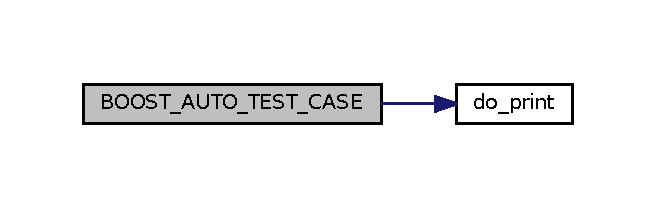
\includegraphics[width=315pt]{test__ip__print_8cpp_ab85b737b15d7ec91dd3b82af8d296f40_cgraph}
\end{center}
\end{figure}


\index{test\+\_\+ip\+\_\+print.\+cpp@{test\+\_\+ip\+\_\+print.\+cpp}!B\+O\+O\+S\+T\+\_\+\+A\+U\+T\+O\+\_\+\+T\+E\+S\+T\+\_\+\+C\+A\+SE@{B\+O\+O\+S\+T\+\_\+\+A\+U\+T\+O\+\_\+\+T\+E\+S\+T\+\_\+\+C\+A\+SE}}
\index{B\+O\+O\+S\+T\+\_\+\+A\+U\+T\+O\+\_\+\+T\+E\+S\+T\+\_\+\+C\+A\+SE@{B\+O\+O\+S\+T\+\_\+\+A\+U\+T\+O\+\_\+\+T\+E\+S\+T\+\_\+\+C\+A\+SE}!test\+\_\+ip\+\_\+print.\+cpp@{test\+\_\+ip\+\_\+print.\+cpp}}
\subsubsection[{\texorpdfstring{B\+O\+O\+S\+T\+\_\+\+A\+U\+T\+O\+\_\+\+T\+E\+S\+T\+\_\+\+C\+A\+S\+E(print\+\_\+test\+\_\+1)}{BOOST_AUTO_TEST_CASE(print_test_1)}}]{\setlength{\rightskip}{0pt plus 5cm}B\+O\+O\+S\+T\+\_\+\+A\+U\+T\+O\+\_\+\+T\+E\+S\+T\+\_\+\+C\+A\+SE (
\begin{DoxyParamCaption}
\item[{print\+\_\+test\+\_\+1}]{}
\end{DoxyParamCaption}
)}\hypertarget{test__ip__print_8cpp_a8ca48550418bc3eaeacd892f6f311f53}{}\label{test__ip__print_8cpp_a8ca48550418bc3eaeacd892f6f311f53}


Here is the call graph for this function\+:
\nopagebreak
\begin{figure}[H]
\begin{center}
\leavevmode
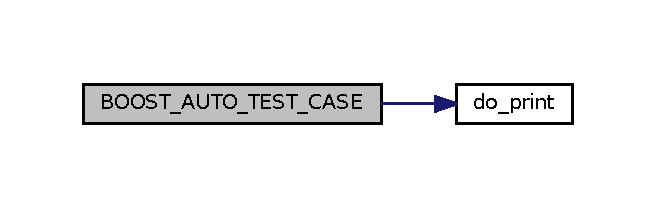
\includegraphics[width=315pt]{test__ip__print_8cpp_a8ca48550418bc3eaeacd892f6f311f53_cgraph}
\end{center}
\end{figure}


\index{test\+\_\+ip\+\_\+print.\+cpp@{test\+\_\+ip\+\_\+print.\+cpp}!B\+O\+O\+S\+T\+\_\+\+A\+U\+T\+O\+\_\+\+T\+E\+S\+T\+\_\+\+C\+A\+SE@{B\+O\+O\+S\+T\+\_\+\+A\+U\+T\+O\+\_\+\+T\+E\+S\+T\+\_\+\+C\+A\+SE}}
\index{B\+O\+O\+S\+T\+\_\+\+A\+U\+T\+O\+\_\+\+T\+E\+S\+T\+\_\+\+C\+A\+SE@{B\+O\+O\+S\+T\+\_\+\+A\+U\+T\+O\+\_\+\+T\+E\+S\+T\+\_\+\+C\+A\+SE}!test\+\_\+ip\+\_\+print.\+cpp@{test\+\_\+ip\+\_\+print.\+cpp}}
\subsubsection[{\texorpdfstring{B\+O\+O\+S\+T\+\_\+\+A\+U\+T\+O\+\_\+\+T\+E\+S\+T\+\_\+\+C\+A\+S\+E(print\+\_\+test\+\_\+2)}{BOOST_AUTO_TEST_CASE(print_test_2)}}]{\setlength{\rightskip}{0pt plus 5cm}B\+O\+O\+S\+T\+\_\+\+A\+U\+T\+O\+\_\+\+T\+E\+S\+T\+\_\+\+C\+A\+SE (
\begin{DoxyParamCaption}
\item[{print\+\_\+test\+\_\+2}]{}
\end{DoxyParamCaption}
)}\hypertarget{test__ip__print_8cpp_aea4481282587bde1a22312b47799faf1}{}\label{test__ip__print_8cpp_aea4481282587bde1a22312b47799faf1}


Here is the call graph for this function\+:
\nopagebreak
\begin{figure}[H]
\begin{center}
\leavevmode
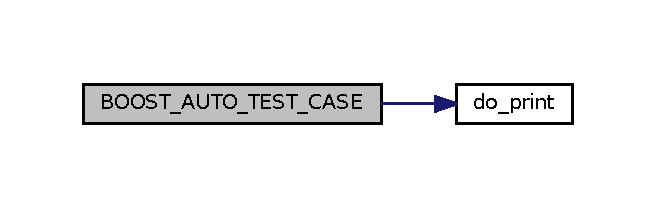
\includegraphics[width=315pt]{test__ip__print_8cpp_aea4481282587bde1a22312b47799faf1_cgraph}
\end{center}
\end{figure}


\index{test\+\_\+ip\+\_\+print.\+cpp@{test\+\_\+ip\+\_\+print.\+cpp}!B\+O\+O\+S\+T\+\_\+\+A\+U\+T\+O\+\_\+\+T\+E\+S\+T\+\_\+\+C\+A\+SE@{B\+O\+O\+S\+T\+\_\+\+A\+U\+T\+O\+\_\+\+T\+E\+S\+T\+\_\+\+C\+A\+SE}}
\index{B\+O\+O\+S\+T\+\_\+\+A\+U\+T\+O\+\_\+\+T\+E\+S\+T\+\_\+\+C\+A\+SE@{B\+O\+O\+S\+T\+\_\+\+A\+U\+T\+O\+\_\+\+T\+E\+S\+T\+\_\+\+C\+A\+SE}!test\+\_\+ip\+\_\+print.\+cpp@{test\+\_\+ip\+\_\+print.\+cpp}}
\subsubsection[{\texorpdfstring{B\+O\+O\+S\+T\+\_\+\+A\+U\+T\+O\+\_\+\+T\+E\+S\+T\+\_\+\+C\+A\+S\+E(print\+\_\+test\+\_\+3)}{BOOST_AUTO_TEST_CASE(print_test_3)}}]{\setlength{\rightskip}{0pt plus 5cm}B\+O\+O\+S\+T\+\_\+\+A\+U\+T\+O\+\_\+\+T\+E\+S\+T\+\_\+\+C\+A\+SE (
\begin{DoxyParamCaption}
\item[{print\+\_\+test\+\_\+3}]{}
\end{DoxyParamCaption}
)}\hypertarget{test__ip__print_8cpp_a9b40e7c2532d72552ef6dc03f800d2e4}{}\label{test__ip__print_8cpp_a9b40e7c2532d72552ef6dc03f800d2e4}


Here is the call graph for this function\+:
\nopagebreak
\begin{figure}[H]
\begin{center}
\leavevmode
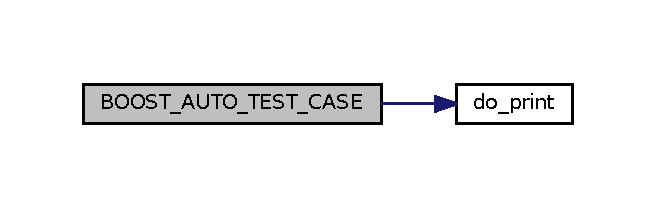
\includegraphics[width=315pt]{test__ip__print_8cpp_a9b40e7c2532d72552ef6dc03f800d2e4_cgraph}
\end{center}
\end{figure}



%--- End generated contents ---

% Index
\backmatter
\newpage
\phantomsection
\clearemptydoublepage
\addcontentsline{toc}{chapter}{Index}
\printindex

\end{document}
